\documentclass[one column]{report}
\usepackage[utf8]{inputenc}

\usepackage{amsmath,amsthm,amssymb}

\usepackage{subcaption}
\usepackage{graphicx}

\usepackage{diagbox}

\usepackage{biblatex}

\bibliography{ref}

\graphicspath{{./images/}}

\usepackage{listings}


\usepackage{color}

\definecolor{gray}{rgb}{0.5,0.5,0.5}
\definecolor{orange}{rgb}{0.8,0,0}

\lstdefinestyle{matlab}{
  belowcaptionskip=1\baselineskip,
  breaklines=true,
  frame=L,
  xleftmargin=\parindent,
  language=octave,
  showstringspaces=false,
  basicstyle=\footnotesize\ttfamily,
  keywordstyle=\bfseries\color{green},
  commentstyle=\color{gray},
  identifierstyle=\color{blue},
  stringstyle=\color{orange},
}
\lstdefinestyle{R}{
  belowcaptionskip=1\baselineskip,
  breaklines=true,
  frame=L,
  xleftmargin=\parindent,
  language=R,
  showstringspaces=false,
  basicstyle=\footnotesize\ttfamily,
  keywordstyle=\bfseries\color{green},
  commentstyle=\color{gray},
  identifierstyle=\color{blue},
  stringstyle=\color{orange},
}

\def\listingsfont{\ttfamily} 
\def\listingsfontinline{\ttfamily}

\title{TAMS39 - Examination exercises}
\author{Anton Karlsson\\antka388\\931217-7117}
\date{}
\begin{document}
\maketitle

\section*{Exercise 1}

\subsection*{(a)}
\label{sec:a}

Let $H_0: \mu_{\rm female}= \mu_{\rm male}$ against $A \neq H$. The
using Hotelling's $T^2$ test, we find that $H_0$ cannot be rejected in
favor of $A$. Thus we may put $\mu = \mu_{\rm female} = \mu_{\rm male}$.

\subsection*{(b)}
\label{sec:b}

Using \texttt{matlab}, we could plot the confidence ellipse around
${\bf \mu}$, see Figure \ref{fig:ex1-ellipse}.
\begin{figure}[h]
  \centering
  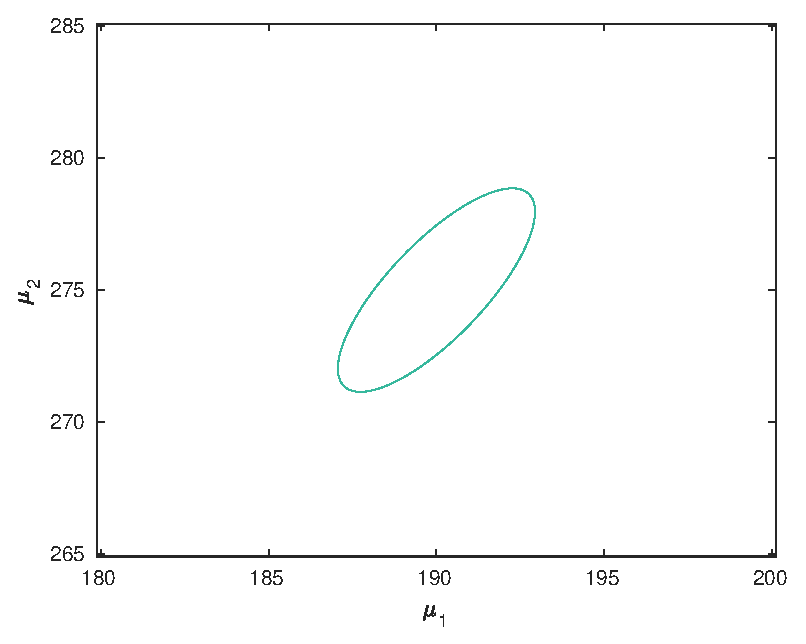
\includegraphics[width=5cm]{ellipse-ex1}
  \caption{The confidence ellipse around ${\bf \mu}$.}
  \label{fig:ex1-ellipse}
\end{figure}

\subsection*{(c)}
\label{sec:c}

Using $a_1 = (1,0)^T$ and $a_2 = (0,1)^T$, we find that the confidence
interval around $\mu_1$ is given by
\begin{equation*}
  \left(
    a \pm T_{1-\alpha} \sqrt{\frac{a_i^T S a_1i^T}{n}}
  \right), \quad i = 1,2,
\end{equation*}
with $T_{1-\alpha} = \frac{n-p}{p(n-1)}F_{1-\alpha}(p, n-p)$. Thus we
get the confidence intervals
\begin{align*}
  (184.7356&,\ 195.2644),\quad i = 1, \\
  (268.0801&,\ 281.9199),\quad i = 2.
\end{align*}


%%% Local Variables:
%%% mode: latex
%%% TeX-master: "examination"
%%% End:


\section*{Exercise 2}
\label{sec:exercise-2}

\subsection*{(a)}
\label{sec:a-1}

The scatter plot can be found in Figure \ref{fig:ex2-scatter} the outlier can be
clearly be seen at $x_1 = 284$.
\begin{figure}[h]
  \centering
  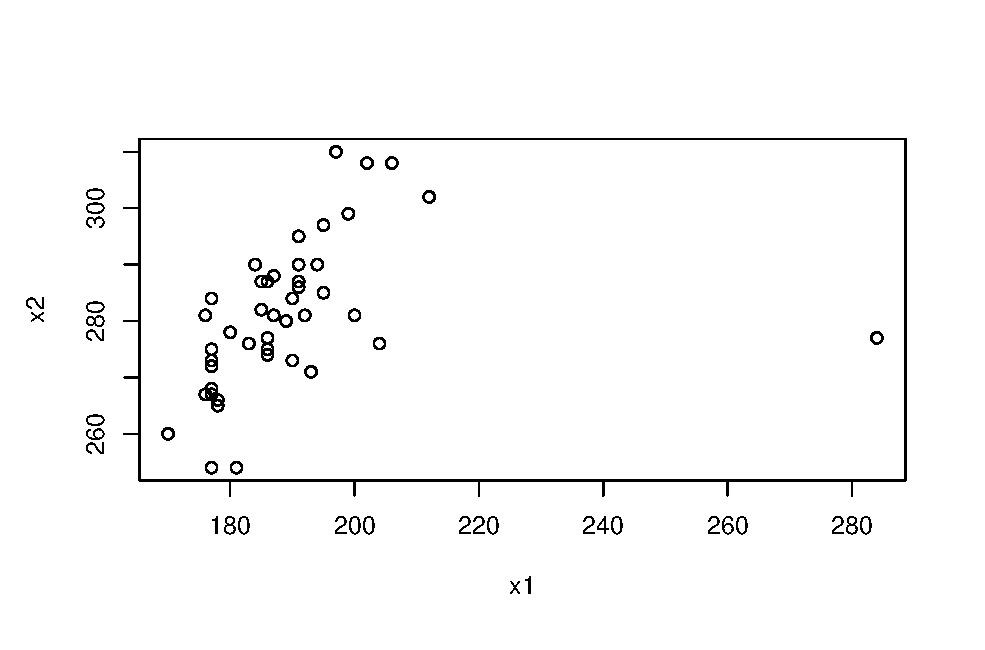
\includegraphics[width=5cm]{ex2-scatterplot}
  \caption{Scatter plot of the tail length and the wing span for male
    hook-billed kites.}
  \label{fig:ex2-scatter}
\end{figure}

\subsection*{(b)}
\label{sec:b-1}

Using the Box corrected test found in \cite[p. 311]{book}, we find that
we can not pool the covariance matrices (see code for details).

\subsection*{(c)}
\label{sec:c-1}

In this test, the pooled matrix $S_p$ was used. Using the Hotelling's
$T^2$ test, we can put $\delta = \bar{x}_{\rm male}- \bar{x}_{\rm
  female}$, we can use the test variable
\begin{equation*}
  T^2 = \frac{n_{\rm female}  n_{\rm male}}{n_{\rm female} +  n_{\rm male}}\delta^T S_p^{-1}\delta,
  \label{eq:1}
\end{equation*}
and rejected $H_0: \mu_{\rm male} = \mu_{\rm female}$ if the test
variable is larger than
\begin{equation*}
 c  = \frac{fp}{f-p+1}F_{1-\alpha}(p, n-p), %c = f*p*qf(1-0.05, p, f-p)/(f-p+1)
\end{equation*}
where $f = n - 1$, and $p = 2$. Since $T^2 = 7.494772$ and $c =
6.27986$, we reject $H_0: \mu_{\rm male} = \mu_{\rm female} $.

The result would most likely hold if we changed the value of the
outlier to $x_1 = 184$ instead of 284, since the sample size should be too
large enough for any drastic changes in the variance matrix or mean to
happen.

\subsection*{(d)}
\label{sec:d}
??

\subsection*{(e)}
\label{sec:e}

The confidence region if given by the equation, for $\mu = (\mu_1, \mu_2).$
\begin{equation}
  \label{eq:ex2-conf-region}
 \{\mu:\ n (\delta - \mu)^T S_p^{-1} (\delta-\mu)\leq \frac{(n-1)p}{n-p}F_{1-\alpha}(p,n-p)\},
\end{equation}
where $\alpha = 0.05$, $S_p$ is the pooled matrix from the previous
exercise, and $\delta = \bar{x}_{\rm male}  - \bar{x}_{\rm
  female}$. Computing the LHS of \eqref{eq:ex2-conf-region}, get
\begin{align*}
  89
  \big(
    &206.7294 ( - 6.463131 -\mu_1)^2 + 189.1233(1.176768 -\mu_2)^2 \\
    &+ 202.2905(- 6.463131 - \mu_1)(1.176768- \mu_2)
  \big)\\
  &\leq \frac{88\cdot 2}{87}3.103839
\end{align*}
Further, to find the confidence intervals for the the different
components, we use the vectors $a_1 = (1,0)^T$ and $a_2 = (0,1)^T$, to
create each of the component wise intervals, respectively. The
intervals, for each $a$, is given by 
\begin{equation*}
  n_f n_m \delta^T S_p^{-1} \delta / (n_f + n_m) , 
\end{equation*}
where.
we get the intervals
\begin{align*}
  (-170.698117786475&; 157.771855160212), \quad \text{for } a = (1,0)
  \\
  (-149.071120157853&;151.424655511388), \quad \text{for } a = (0,1)
\end{align*}

\subsection*{(f)}
\label{sec:f}

From the interval we find the Exercise (e), we see that there are no
genrall difference for the lengths between the female and the male birds.
\subsection*{\texttt{R} code}
\label{sec:textttr-code}

\lstinputlisting[style=R]{../ex2.R}

%%% Local Variables:
%%% mode: latex
%%% TeX-master: "examination"
%%% End:

\section*{Exercise 3}
\label{sec:exercise-3}

\subsection*{(a)}
\label{sec:a-2}
The plot of the profiles are presented in figure
\ref{fig:ex3-profiles}.
\begin{figure}[h]
  \centering
  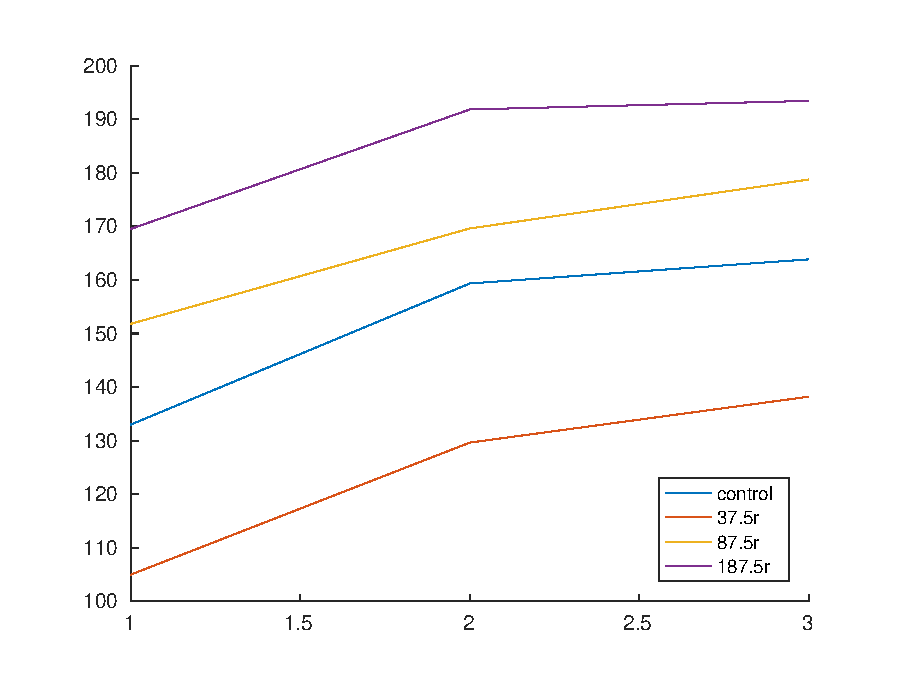
\includegraphics[width=8.5cm]{ex3-profiles}
  \caption{The profiles for the Psychomotor scores given different
    radiation treatment.}
  \label{fig:ex3-profiles}
\end{figure}

\subsection*{(b)}
\label{sec:b-2}

%Check the updated code, which should probably correct. 

To test if the profiles are parallel the test presented in Lecture
7 is used. First we introduce the matrices
\begin{align*}
  \b A &=
         \begin{pmatrix}
           \b 1_{n_{1}}  & \b 0_{n_{1}}& \b 0_{n_{1}}& \b 0_{n_{1}} \\
           \b 0_{n_{2}} &  \b 1_{n_{2}}  &\b 0_{n_{2}}& \b 0_{n_{2}} \\
           \b 0_{n_{3}}& \b 0_{n_{3}}&  \b 1_{n_{3}}  & \b 0_{n_{3}} \\
           \b 0_{n_{4}}& \b 0_{n_{4}}& \b 0_{n_{4}} &   \b 1_{n_{4}}   \\ 
         \end{pmatrix} \\
  \b V &= \b X^{T} (\b I_{n}   -  \b A(\b A^{T}\b A)^{-1}\b A^{T}) \b X, \\
  \b C &=
         \begin{pmatrix}
           1 & -1 & 0 \\
           1 &  0 & -1
         \end{pmatrix}, \\
  \b Y &=
         \begin{pmatrix}
           \b \mu_{1} - \mu_{4} &\b \mu_{2} - \mu_{4} &\b \mu_{3} - \mu_{4} 
         \end{pmatrix} \\
  \b C_{Y}^{-1} &= \diag (n_{1}, n_{2}, n_{3}) - \frac{1}{n}   (n_{1},
                  n_{2}, n_{3})^{T} (n_{1}, n_{2}, n_{3}), \\
  \b H &= \b Y\b C_{Y}^{-1}\b Y^{T}                  
\end{align*}
Then we construct the test statistic
\begin{equation*}
  Q = -
  \left(
    n - \frac{1}{2}(k + p + 1)
  \right)
  \left(
    \ln \abs{\b {CVC}^{T}} - \ln \abs{\b{CVC}^{T} + \b{CHC}^{T}}
  \right) ,
\end{equation*}
where we reject $H_{1}: $ \textit{the profiles are parallel} if $Q$ is larger
than 
\begin{equation*}
  c = \chi^{2}_{(p-1)(k-1)}(1 - \alpha), \quad \alpha = 0.05.
\end{equation*}
Since $Q =4.0443 $ and $c = 12.5916$, we cannot reject $H_{1}$, the
profiles are parallel


\subsection*{(c)}
\label{sec:c-2}

Since, the profiles are parallel, we can set up a test for checking if
the profiles are on the same level. The likelihood ratio is 
\begin{equation*}
  \lambda_{H_2 | H_1} = \frac{\abs{\b C\b V \b C^{T} + \b C \b H\b C^T}}{\abs{\b
      C\b V \b C^T}}\frac{\abs{\b V}}{\abs{\b V+\b H}},
\end{equation*}
from which $H_{2}|H_{1}$ is rejected if 
\begin{equation*}
  Q = \left(\frac{n-k - p +1}{k - 1}\right)\frac{1 - \lambda_{H_2 |H_1}}{\lambda_{H_2 | H_1}},
\end{equation*}
is larger then 
\begin{equation*}
  c = F_{k-1, n - k - p +1} (1 - \alpha), \quad \alpha = 0.05
\end{equation*}
We get
\begin{equation*}
 7.9361  = Q < c = 3.2145,
\end{equation*}
so $H_2 | H_1$ is rejected, the profiles are not on the same level.

\subsection*{(d)}
\label{sec:d-1}

Here, we use the test variables 
\begin{equation*}
  \lambda_{H_3 | H_1} = \frac{1}{1 + n \bar{\bf x}^T \b C^T (\b{CVC}^T +
    \b{CHC}^T)^{-1}}\b C\bar{\bf x},
\end{equation*}
and create the test variable
\begin{equation*}
  Q = \frac{n - p +1}{p - 1}\lambda_{H_3 |H_1}, 
\end{equation*}
which we compare to 
\begin{equation*}
  c = F_{p-1, n-p+1}(0.95).
\end{equation*}
We get
\begin{equation*}
  7.9361 = Q > c = 3.2145.
\end{equation*}
Thus $H_3 | H_1$ is rejected, the profiles are not flat.
%%% Local Variables:
%%% mode: latex
%%% TeX-master: "examination"
%%% End:

\section*{Exercise 4}
\label{sec:exercise-4}

\subsection*{(a)}
\label{sec:a-3}

To check if the covariance matrices can be pooled, the hypothesis
$H_{0}: \Sigma_{1} =\Sigma_{2}  = \Sigma_{3}$ is considered. We
reject $H_{0}$ if
\begin{equation*}
  \Lambda^* = \frac{\prod_{i = 1}^{3} \abs{\b V_i}^{f_i/2}}{\abs{\b V}^{f/2}}
  \frac{f^{pf/2}}{\prod_{i = 1}^{3} f_i ^{pf_{i}/2}} < c,\quad
  \text{for some } c,
\end{equation*}
where $f_{i} = n_{i} - 1$, are the degrees of freedom for group $i = 1,
2, 3$, $f = \sum_{i=1}^{3}f_{i}$, and
\begin{equation*}
  \b V_{i} = \b X_{i} (\b I_{n_{i}}  - \frac 1n_{i}\b 1_{n_{i}} \b 1_{n_{i}}^{T})^{T}
  \b X_{i}^{T},\quad i = 1,2,3,
\end{equation*}
and
\begin{equation*}
  \b V = \sum_{i=1}^{3} \b V_{i}.
\end{equation*}
The test $\Lambda^{*} < c$, for some $c$, is an unbiased test.
Further, we can use the correction found in Lecture 5, where
\begin{equation*}
  -2 \frac{m}{f} \ln \Lambda^{*} \sim \chi^{2}(df), \quad df = \frac{1}{2}p(p+1)(r-1),
\end{equation*}
where $m = f- 2\alpha$, where
\begin{equation*}
  \alpha = 
  \left(
    \sum_{i = 1}^{3} \frac{f}{f_{i}} - 1
  \right)
  \frac{2p^{2} + p -1}{12(p+1)(3-1)}.
\end{equation*}
Then 
\begin{equation*}
   -2 \frac{m}{f} \ln \Lambda^{*} = 49.26
\end{equation*}
and
\begin{equation*}
  \chi_{df}^{2}(1-\alpha) = 91.670, \quad \alpha = 0.05,
\end{equation*}
hence $H_{0}$ cannot be rejected, the covariance matrices can be
pooled. 
\subsection*{(b)}
\label{sec:b-3}

Since we can pool the sample matrix, which is given as
\begin{equation*}
  \b S_{\rm spooled} =
  \begin{pmatrix}
    156.82 &57.13 &20.27 &22.13 &0.16 &20.40 \\ 
    57.13 &53.20 &10.93 &9.57 &-0.47 &11.67 \\ 
    20.27 &10.93 &5.95 &6.30 &-0.23 &4.67 \\ 
    22.13 &9.57 &6.30 &22.39 &-0.54 &11.37 \\ 
    0.16 &-0.47 &-0.23 &-0.54 &0.99 &0.06 \\ 
    20.40 &11.67 &4.67 &11.37 &0.06 &53.09 
  \end{pmatrix},
\end{equation*}
we can use the distance function $d_{i}(\b x_{0}) = (\b x_{0} - \mean
x_{i})^{T} \b S_{\rm spooled}^{-1} (\b x_{0} - \mean
x_{i})$ given in \cite[p. 611]{book}, where  $\b x_{0}$ is classified to
$\pi_{i}$ if $d_{i}(\b x_{0}) = \min_{i = 1, 2, 3}
\left\{
    d_{i}(\b x_{0})
\right\}$. The distance functions can be created with
\begin{equation*}
  S_{\rm pooled}^{-1} =
  \begin{pmatrix}
    0.01 &-0.01 &-0.03 &-0.00 &-0.01 &-0.00 \\ 
    -0.01 &0.04 &-0.04 &0.01 &0.01 &-0.00 \\ 
    -0.03 &-0.04 &0.42 &-0.07 &0.04 &-0.00 \\ 
    -0.00 &0.01 &-0.07 &0.07 &0.03 &-0.01 \\ 
    -0.01 &0.01 &0.04 &0.03 &1.05 &-0.01 \\ 
    -0.00 &-0.00 &-0.00 &-0.01 &-0.01 &0.02  
  \end{pmatrix},
\end{equation*}
and 
\begin{equation*}
  \mean x_{1} =
  \begin{pmatrix}
    183.10 \\ 
    129.62 \\ 
    51.24 \\ 
    146.19 \\ 
    14.10 \\ 
    104.86 
  \end{pmatrix}, \quad 
  \mean x_{2} =
  \begin{pmatrix}
    201.00 \\ 
    119.32 \\ 
    48.87 \\ 
    124.65 \\ 
    14.29 \\ 
    81.00  
  \end{pmatrix}, \quad 
  \mean x_{3} =
  \begin{pmatrix}
    138.23 \\ 
    125.09 \\ 
    51.59 \\ 
    138.27 \\ 
    10.09 \\ 
    106.59
  \end{pmatrix}.
\end{equation*}



\subsection*{(c)}
\label{sec:c-3}
Since both the means and the varaince is unkown, we use the estimates
of the errors of missclassification according to Okamato. First define 
\begin{align*}
  a_{1} &= \frac{\hat\Delta^{2} +
    12(p-1)}{16\hat\Delta}\phi(\hat\Delta) =0.99 ,  \quad a_{2} =
  \frac{\hat\Delta^{2} + 4(p-1)}{16\hat\Delta}\phi(\hat\Delta) =0.18 , \quad
  \text{and}\quad \\
  a_{3} &= \frac{\hat\Delta(p-1)}{4}\phi(\hat\Delta) = 7.70,
\end{align*}
where 
\begin{equation*}
  \hat\Delta^{2} = \frac{f - p - 1}{f} (\mean x_{1} - \mean x_{2})^{T}
  \b S_{\rm pooled}^{-1} (\mean x_{1} - \mean x_{2}) = 6.16,
  \quad f = n_{1} + n_{2} - 2 = 50.
\end{equation*}
Then the error of missclassificating a member of $\pi_{0}$ onto 
$\pi_{1}$ is given by 
\begin{equation*}
  e_{1} = P(\b x_{0} \in \pi_{2}) \approx  \phi(-\frac 12 \hat\Delta) + \frac{a_{1}}{n_{1}} +
  \frac{a_{2}}{n_{2}} + \frac{a_{3}}{f} = 0.21,  
\end{equation*}
and the error of missclassificating a member of $\pi_{0}$ onto 
$\pi_{2}$ is
\begin{equation*}
  e_{1} = P(\b x_{0} \in \pi_{1}) \approx  \phi(-\frac 12 \hat\Delta) + \frac{a_{2}}{n_{1}} +
  \frac{a_{1}}{n_{2}} + \frac{a_{3}}{f} = 0.20.
\end{equation*}

%%% Local Variables:
%%% mode: latex
%%% TeX-master: "examination"
%%% End:


\begin{comment}
  
  We could calculate the linear separators, $ l_i^T x_0 + c_i$, where
  we obtain
  \begin{align*}
    l_1^T x_0 + c_1 &= (-0.57, 1.80, 1.01, 6.33, 18.94, 0.33)x_0 + -703.95 \\ 
    l_2^T x_0 + c_2 &= (-0.14, 1.31, 1.48, 5.15, 18.31, 0.04)x_0 + -554.06 \\ 
    l_3^T x_0 + c_3 &= (-1.08, 1.89, 3.03, 5.69, 15.11, 0.51)x_0 + -618.43,
  \end{align*}
  In which we can conclude that ${\bf x_0}$ belongs to  $\pi_i$ if $
  l_i^T x_0 + c_i = \max_i \left(   l_i^T x_0 + c_i\right)
  $

\end{comment}

\section*{Exercise 5}
\label{sec:exercise5}

\subsection*{(a)}
\label{sec:a-4}

The dot diagrams\footnote{Jag är lite osäker på hur dot diagram ska se
  ut. Och framföralt hur man gjorde ett i \texttt{matlab}, men jag
  hoppas att detta illusterar det du är ute efter.} are shown in Figure \ref{fig:ex5-marginalplots}. 

\begin{figure}[h]
  \centering
  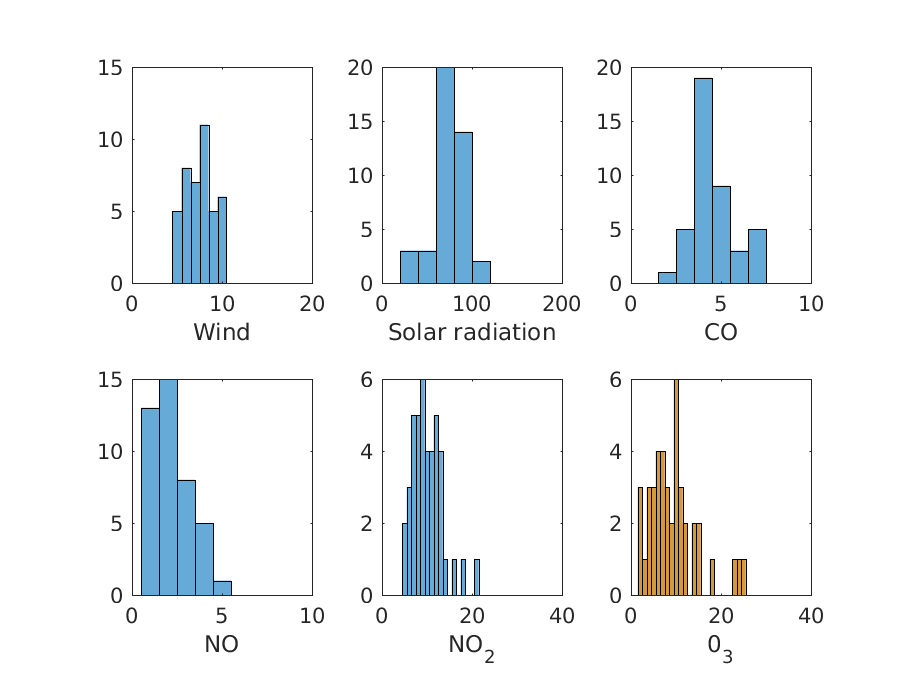
\includegraphics[width=13cm]{ex5-marginalplots}
  \caption{The marginal dot diagrams for all variables}
  \label{fig:ex5-marginalplots}
\end{figure}

\subsection*{(b)}
\label{sec:b-4}

The sample mean is given as
\begin{equation*}
  \bar{x} =
  \begin{pmatrix}
    7.50 & 73.86 & 4.55 & 2.19 & 10.05 & 9.40 & 3.10 
  \end{pmatrix}^T
\end{equation*}
and
\begin{equation*}
  S =
  \begin{pmatrix}
    2.50 & -2.78 & -0.38 & -0.46 & -0.59 & -2.23 & 0.17 \\ 
    -2.78 & 300.52 & 3.91 & -1.39 & 6.76 & 30.79 & 0.62 \\ 
    -0.38 & 3.91 & 1.52 & 0.67 & 2.31 & 2.82 & 0.14 \\ 
    -0.46 & -1.39 & 0.67 & 1.18 & 1.09 & -0.81 & 0.18 \\ 
    -0.59 & 6.76 & 2.31 & 1.09 & 11.36 & 3.13 & 1.04 \\ 
    -2.23 & 30.79 & 2.82 & -0.81 & 3.13 & 30.98 & 0.59 \\ 
    0.17 & 0.62 & 0.14 & 0.18 & 1.04 & 0.59 & 0.48 \\ 
  \end{pmatrix}
\end{equation*}

\subsection*{(c)}
\label{sec:c-4}

The model used was
\begin{equation*}
  y_1 = \beta_0 + \beta_1 x_1 + \beta_2 x_2 + \epsilon,
\end{equation*}
where $\hat{\beta} = (10.1145,\   -0.2113,\    0.0205)$. From here we
can calculate the residual:
\begin{equation*}
  \text{SS}_{\rm E} = 455.1356.
\end{equation*}

Further, we got the following confidence interval with confidence level of 95
\%: $(7.59, 11.71)$. 

\subsection*{(d)}

Here, we propose the linear model
\begin{equation*}
  \begin{pmatrix}
    y_1 \\ y_2
  \end{pmatrix} = 
  BX + E,
\end{equation*}
where 
\begin{equation*}
  X =
  \begin{pmatrix}
    {\bf 1_n} & x_2 & x_2
  \end{pmatrix}.
\end{equation*}
We found that
\begin{equation*}
  B =
  \begin{pmatrix}
    10.11 & -0.21 \\ 
    0.02 & 8.28 \\ 
    -0.79 & 0.10 
  \end{pmatrix}.
\end{equation*}

The confidence region for $x_1 = 10$ and $x_2 = 80$ is shown in Figure
\ref{fig:ex5-ellipse}
\begin{figure}[h]
  \centering
  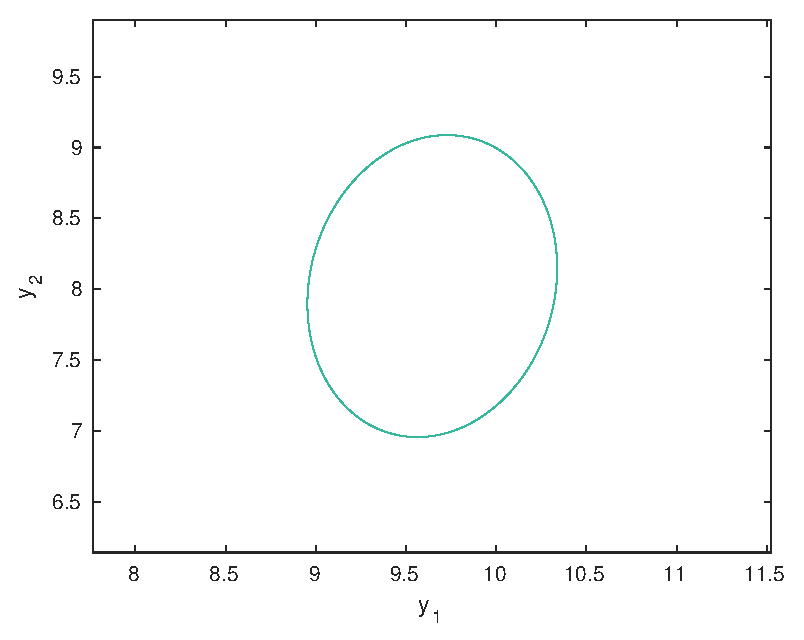
\includegraphics[width=7cm]{ex5-ellipse}
  \caption{The confidence region for $x_1 = 10$ and $x_2 = 80$. }
  \label{fig:ex5-ellipse}
\end{figure}

We can see that the ellipse is covered by 
the confidence interval in Exercise~(c), on the $y_1$ axis.

%%% Local Variables:
%%% mode: latex
%%% TeX-master: "examination"
%%% End:


\printbibliography

\end{document}
%%% Local Variables:
%%% mode: latex
%%% TeX-master: t
%%% End:
